% Created by tikzDevice version 0.12.6 on 2026-08-03 04:29:02
% !TEX encoding = UTF-8 Unicode
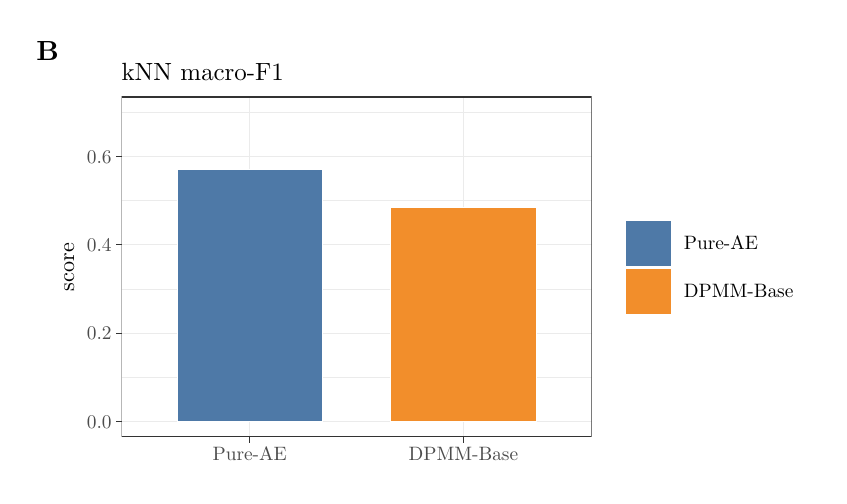
\begin{tikzpicture}[x=1pt,y=1pt]
\definecolor{fillColor}{RGB}{255,255,255}
\path[use as bounding box,fill=fillColor,fill opacity=0.00] (0,0) rectangle (285.80,161.83);
\begin{scope}
\path[clip] (  1.11,  1.74) rectangle (284.69,160.09);
\definecolor{drawColor}{RGB}{255,255,255}
\definecolor{fillColor}{RGB}{255,255,255}

\path[draw=drawColor,line width= 0.4pt,line join=round,line cap=round,fill=fillColor] (  1.11,  1.74) rectangle (284.69,160.09);
\end{scope}
\begin{scope}
\path[clip] ( 33.93, 13.93) rectangle (203.76,136.79);
\definecolor{fillColor}{RGB}{255,255,255}

\path[fill=fillColor] ( 33.93, 13.93) rectangle (203.76,136.79);
\definecolor{drawColor}{gray}{0.92}

\path[draw=drawColor,line width= 0.2pt,line join=round] ( 33.93, 35.47) --
	(203.76, 35.47);

\path[draw=drawColor,line width= 0.2pt,line join=round] ( 33.93, 67.38) --
	(203.76, 67.38);

\path[draw=drawColor,line width= 0.2pt,line join=round] ( 33.93, 99.30) --
	(203.76, 99.30);

\path[draw=drawColor,line width= 0.2pt,line join=round] ( 33.93,131.21) --
	(203.76,131.21);

\path[draw=drawColor,line width= 0.4pt,line join=round] ( 33.93, 19.52) --
	(203.76, 19.52);

\path[draw=drawColor,line width= 0.4pt,line join=round] ( 33.93, 51.43) --
	(203.76, 51.43);

\path[draw=drawColor,line width= 0.4pt,line join=round] ( 33.93, 83.34) --
	(203.76, 83.34);

\path[draw=drawColor,line width= 0.4pt,line join=round] ( 33.93,115.25) --
	(203.76,115.25);

\path[draw=drawColor,line width= 0.4pt,line join=round] ( 80.25, 13.93) --
	( 80.25,136.79);

\path[draw=drawColor,line width= 0.4pt,line join=round] (157.44, 13.93) --
	(157.44,136.79);
\definecolor{drawColor}{RGB}{255,255,255}
\definecolor{fillColor}{RGB}{78,121,167}

\path[draw=drawColor,line width= 0.3pt,fill=fillColor] ( 54.00, 19.52) rectangle (106.49,110.78);
\definecolor{fillColor}{RGB}{242,142,43}

\path[draw=drawColor,line width= 0.3pt,fill=fillColor] (131.20, 19.52) rectangle (183.69, 96.90);
\definecolor{drawColor}{gray}{0.20}

\path[draw=drawColor,line width= 0.4pt,line join=round,line cap=round] ( 33.93, 13.93) rectangle (203.76,136.79);
\end{scope}
\begin{scope}
\path[clip] (  0.00,  0.00) rectangle (285.80,161.83);
\definecolor{drawColor}{gray}{0.30}

\node[text=drawColor,anchor=base east,inner sep=0pt, outer sep=0pt, scale=  0.70] at ( 30.33, 17.11) {0.0};

\node[text=drawColor,anchor=base east,inner sep=0pt, outer sep=0pt, scale=  0.70] at ( 30.33, 49.02) {0.2};

\node[text=drawColor,anchor=base east,inner sep=0pt, outer sep=0pt, scale=  0.70] at ( 30.33, 80.93) {0.4};

\node[text=drawColor,anchor=base east,inner sep=0pt, outer sep=0pt, scale=  0.70] at ( 30.33,112.84) {0.6};
\end{scope}
\begin{scope}
\path[clip] (  0.00,  0.00) rectangle (285.80,161.83);
\definecolor{drawColor}{gray}{0.20}

\path[draw=drawColor,line width= 0.4pt,line join=round] ( 31.93, 19.52) --
	( 33.93, 19.52);

\path[draw=drawColor,line width= 0.4pt,line join=round] ( 31.93, 51.43) --
	( 33.93, 51.43);

\path[draw=drawColor,line width= 0.4pt,line join=round] ( 31.93, 83.34) --
	( 33.93, 83.34);

\path[draw=drawColor,line width= 0.4pt,line join=round] ( 31.93,115.25) --
	( 33.93,115.25);
\end{scope}
\begin{scope}
\path[clip] (  0.00,  0.00) rectangle (285.80,161.83);
\definecolor{drawColor}{gray}{0.20}

\path[draw=drawColor,line width= 0.4pt,line join=round] ( 80.25, 11.93) --
	( 80.25, 13.93);

\path[draw=drawColor,line width= 0.4pt,line join=round] (157.44, 11.93) --
	(157.44, 13.93);
\end{scope}
\begin{scope}
\path[clip] (  0.00,  0.00) rectangle (285.80,161.83);
\definecolor{drawColor}{gray}{0.30}

\node[text=drawColor,anchor=base,inner sep=0pt, outer sep=0pt, scale=  0.70] at ( 80.25,  5.51) {Pure-AE};

\node[text=drawColor,anchor=base,inner sep=0pt, outer sep=0pt, scale=  0.70] at (157.44,  5.51) {DPMM-Base};
\end{scope}
\begin{scope}
\path[clip] (  0.00,  0.00) rectangle (285.80,161.83);
\definecolor{drawColor}{RGB}{0,0,0}

\node[text=drawColor,rotate= 90.00,anchor=base,inner sep=0pt, outer sep=0pt, scale=  0.80] at ( 16.80, 75.36) {score};
\end{scope}
\begin{scope}
\path[clip] (  0.00,  0.00) rectangle (285.80,161.83);
\definecolor{fillColor}{RGB}{255,255,255}

\path[fill=fillColor] (211.76, 54.02) rectangle (282.69, 96.71);
\end{scope}
\begin{scope}
\path[clip] (  0.00,  0.00) rectangle (285.80,161.83);
\definecolor{fillColor}{RGB}{255,255,255}

\path[fill=fillColor] (215.76, 75.36) rectangle (233.11, 92.71);
\definecolor{drawColor}{RGB}{255,255,255}
\definecolor{fillColor}{RGB}{78,121,167}

\path[draw=drawColor,line width= 0.3pt,fill=fillColor] (216.12, 75.72) rectangle (232.75, 92.35);
\end{scope}
\begin{scope}
\path[clip] (  0.00,  0.00) rectangle (285.80,161.83);
\definecolor{fillColor}{RGB}{255,255,255}

\path[fill=fillColor] (215.76, 58.02) rectangle (233.11, 75.36);
\definecolor{drawColor}{RGB}{255,255,255}
\definecolor{fillColor}{RGB}{242,142,43}

\path[draw=drawColor,line width= 0.3pt,fill=fillColor] (216.12, 58.37) rectangle (232.75, 75.01);
\end{scope}
\begin{scope}
\path[clip] (  0.00,  0.00) rectangle (285.80,161.83);
\definecolor{drawColor}{RGB}{0,0,0}

\node[text=drawColor,anchor=base west,inner sep=0pt, outer sep=0pt, scale=  0.70] at (237.11, 81.62) {Pure-AE};
\end{scope}
\begin{scope}
\path[clip] (  0.00,  0.00) rectangle (285.80,161.83);
\definecolor{drawColor}{RGB}{0,0,0}

\node[text=drawColor,anchor=base west,inner sep=0pt, outer sep=0pt, scale=  0.70] at (237.11, 64.28) {DPMM-Base};
\end{scope}
\begin{scope}
\path[clip] (  0.00,  0.00) rectangle (285.80,161.83);
\definecolor{drawColor}{RGB}{0,0,0}

\node[text=drawColor,anchor=base west,inner sep=0pt, outer sep=0pt, scale=  0.90] at ( 33.93,142.78) {kNN macro-F1};
\end{scope}
\begin{scope}
\path[clip] (  0.00,  0.00) rectangle (285.80,161.83);
\definecolor{drawColor}{RGB}{0,0,0}

\node[text=drawColor,anchor=base,inner sep=0pt, outer sep=0pt, scale=  1.00] at (  7.20,150.08) {\bfseries B};
\end{scope}
\end{tikzpicture}
